%\documentstyle[epsf,twocolumn]{jarticle}       %LaTeX2.09�d�l
\documentclass[twocolumn]{jarticle} 
\setlength{\topmargin}{-45pt}
%\setlength{\oddsidemargin}{0cm} 
\setlength{\oddsidemargin}{-7.5mm}
%\setlength{\evensidemargin}{0cm} 
\setlength{\textheight}{24.1cm}
%setlength{\textheight}{25cm} 
\setlength{\textwidth}{17.4cm}
%\setlength{\textwidth}{172mm} 
\setlength{\columnsep}{11mm}

% 【節が変わるごとに (1.1)(1.2) … (2.1)(2.2) と数式番号をつけるとき】
%\makeatletter
%\renewcommand{\theequation}{%
%\thesection.\arabic{equation}} %\@addtoreset{equation}{section}
%\makeatother

%\renewcommand{\arraystretch}{0.95}行間の設定

%%%%%%%%%%%%%%%%%%%%%%%%%%%%%%%%%%%%%%%
\usepackage[dvipdfmx]{graphicx} %pLaTeX2e仕様(\documentstyle ->\documentclass)
\usepackage{url}		%参考文献にurlを入れる用
\usepackage{bm}  	%太字形式のベクトルを使う用
\usepackage{amsmath}	%数式の場合分け用
%%%%%%%%%%%%%%%%%%%%%%%%%%%%%%%%%%%%%%%

\begin{document}

	%bibtex用の設定
	%\bibliographystyle{ujarticle}

	\twocolumn[
		\noindent
		\hspace{1em}
		2021 年 5 月 14 日
		三菱共同研究会議資料
		\hfill
		B4	尾關  拓巳
		\vspace{2mm}
		\hrule
		\begin{center}
			{\Large \bf 進捗報告}
		\end{center}
		\hrule
		\vspace{9mm}
	]


\section{ネルダーミード法}
ネルダーミード法\cite{10.1093/comjnl/7.4.308}は1965年にNelderらが発表した最適化アルゴリズムである.n+1個の頂点からなるn次元の単体を反射,膨張,収縮させながら関数の最小値を探索する.


\section{ネルダーミード法を用いたベンチマーク問題の実験}
	\subsection{実験設定}
		ネルダーミード法の実験設定を表1に示す.
		\begin{table}[htbp]
			\begin{center}
				\caption{ネルダーミード法の実験設定}
				\begin{tabular}{| c | c |} \hline
					変化しない場合の許容回数 & 2000 \\
					変化とみなす閾値 & $10^{-11}$ \\ 
					最大操作数 & 無限 \\
					$\alpha$ & 1.0 \\
					$\gamma$ & 2.0 \\
					$\rho$ & 0.5 \\
					$\sigma$ & 0.5 \\ \hline
					
				\end{tabular}
			\end{center}
		\end{table}
		
		$\bm{x}$の初期位置は0から1のランダムな実数とする.

	\subsubsection{評価関数と制約違反}
		取り扱うベンチマーク問題では制約違反を考慮する必要があり,今実験ではその許容量を$1.0\times10^{-10}$とする.また,制約違反の合計値$V$を用いて式1のようにネルダーミード法の目的関数$F$を定義する.
		\begin{equation}
			F(\bm{x}) = \begin{cases}
				f(\bm{x}) & (V < 1.0\times10^{-10}) \\
				V + 10^7 & (otherwise)
			\end{cases}
		\end{equation}
		ただし,ベンチマークの目的関数を$f$とする.
		
	\subsection{結果}
		表2に実験で得られた最終の目的関数値と制約違反の合計値,図1に目的関数値の推移を示す.縦軸は目的関数の値で,横軸は操作回数である.
		\begin{table}[htbp]
			\begin{center}
				\caption{実験結果}
				\begin{tabular}{| c | c |} \hline
					目的関数値 & 制約違反 \\ \hline 
					4200372.158 &  236.2943965 \\ \hline
				\end{tabular}
			\end{center}
		\end{table}
		\begin{figure}
			\centering
            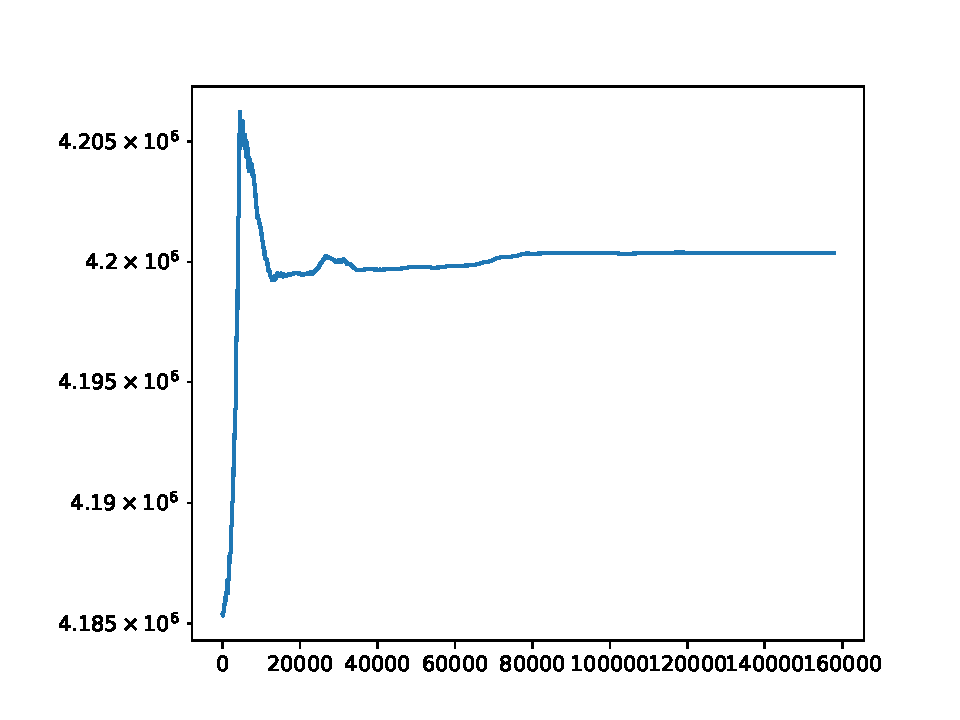
\includegraphics[width=9cm]{nelder.pdf}
            \caption{目的関数値の推移}
        \end{figure}

	表2から,制約違反の合計値が許容量を超えていることがわかる.ネルダーミード法のパラメーターを変えるなど予備実験をしたが,許容量を満たす解を見つけることができなかった.120次元という次元数の高い問題にネルダーミード法が適していないことが原因ではないかと考えた.今実験ではベンチマーク問題の目的関数を式1のように定義し,制約違反が許容量を下回る解を見つけられなかったため,図1は制約違反のみを最小化する際の目的関数値の推移となる.


\section{CMA-ES}
CMA-ES\cite{542381}は1996年にHansenらが発表した,正規分布の共分散行列を学習するCovariance Matrix Adaptation(CMA)を用いた進化型計算である.変数分離不能,悪スケール,多峰性といった困難さをもつ連続最適化問題に対して効率的な探索ができる.

今回は,pythonの進化計算ライブラリであるDEAP\cite{DEAP_JMLR2012}を用いてCMA-ESを実装をした.


\section{CMA-ESを用いたベンチマーク問題の実験}
	\subsection{実験設定}
		表3にCMA-ESの実験設定を示す.
		\begin{table}[htbp]
			\begin{center}
				\caption{CMA-ESの実験設定}
				\begin{tabular}{| c | c |} \hline
					最大世代数 & 6000 \\
					入力次元数 & 120 \\
					1世代あたりの個体数$\lambda$ & 1200 \\
					$\mu$ & 600 \\
					$\sigma^{(0)}$ & 0.05 \\ 
					$\bf{m}^{(0)}$ &  (5,...,5) \\ \hline
				\end{tabular}
			\end{center}
		\end{table}
	

	\subsubsection{制約違反}
	今実験では制約違反の合計値を1つの目的関数$V$とする.またその許容量は$1.0\times10^{-10}$とする.CMA-ESでは,$V$を優先して最小化し許容量以下になった後にベンチマーク問題の目的関数$f$を最小化するように設定する.
	
	\subsection{結果}
		表4に実験で得られた最終の目的関数値と制約違反の合計値,図2に目的関数値の推移を示す.縦軸は目的関数の値で,横軸は世代数である.
		\begin{table}[htbp]
			\begin{center}
				\caption{実験結果}
				\begin{tabular}{| c | c |} \hline
					目的関数値 & 制約違反 \\ \hline 
					4790204.092 &   $9.64638089\times10^{-11}$ \\ \hline
				\end{tabular}
			\end{center}
		\end{table}
		\begin{figure}
			\centering
            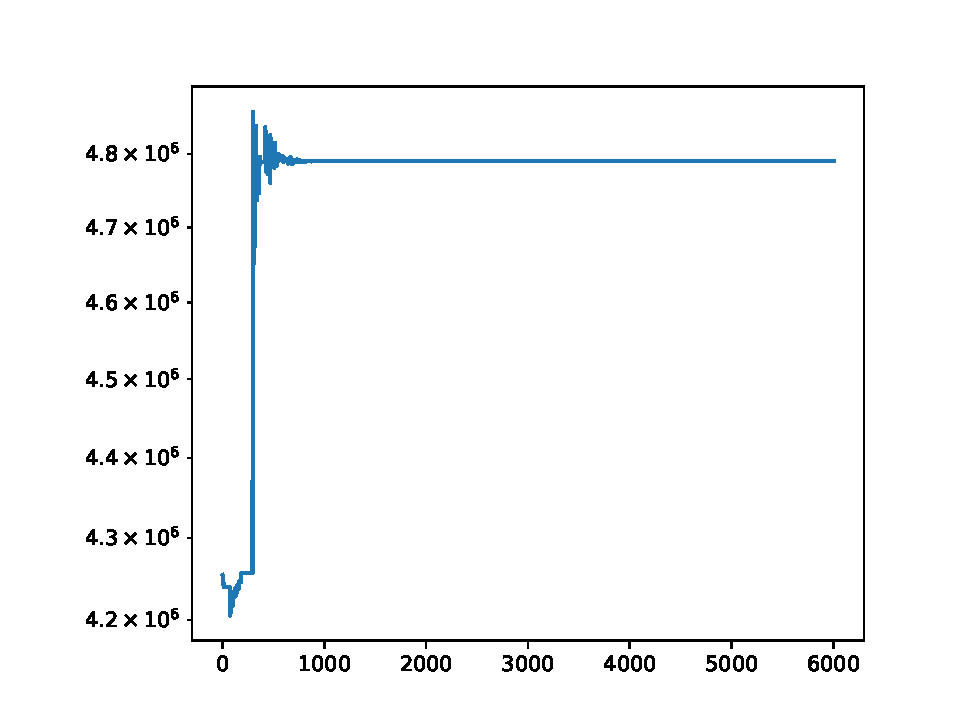
\includegraphics[width=9cm]{cmaes.pdf}
            \caption{目的関数値の推移}
        \end{figure}

		表4より,CMA-ESを用いることで制約違反をクリアする解を見つけることができた.実験においてそのような解は,3005世代目以降から見つかった.最適化の過程で,制約違反を許容量以下に抑えるまでは順調にできたが,目的関数は満足に最適化ができなかった.最適化の最後の方に目的関数が徐々に下がっていく傾向は見られたため,パラメータをうまく調整することで目的関数をさらに最適化できるのではないかと考えた.

\section{ネルダーミード法とCMA-ES}
	ネルダーミード法とCMA-ESを組み合わせた最適化を用いて,ベンチマーク問題について以下の数値実験を行った.
	\begin{itemize}
		\item 実験1: CMA-ESを用いて最適化をし,制約違反を満たす最初の解をネルダーミード法の初期解として代入する.
		\item 実験2: CMA-ESを用いて最適化をし,最終世代の解をネルダーミード法の初期解として代入する.
	\end{itemize}
	実験設定は,ネルダーミード法の変化しない場合の許容回数を4000とする以外は同じである.
	\subsection{実験1}
		図3に結果として得られた目的関数の推移を示す.縦軸は目的関数値,横軸は世代数または操作回数である.
		\begin{figure}
			\centering
            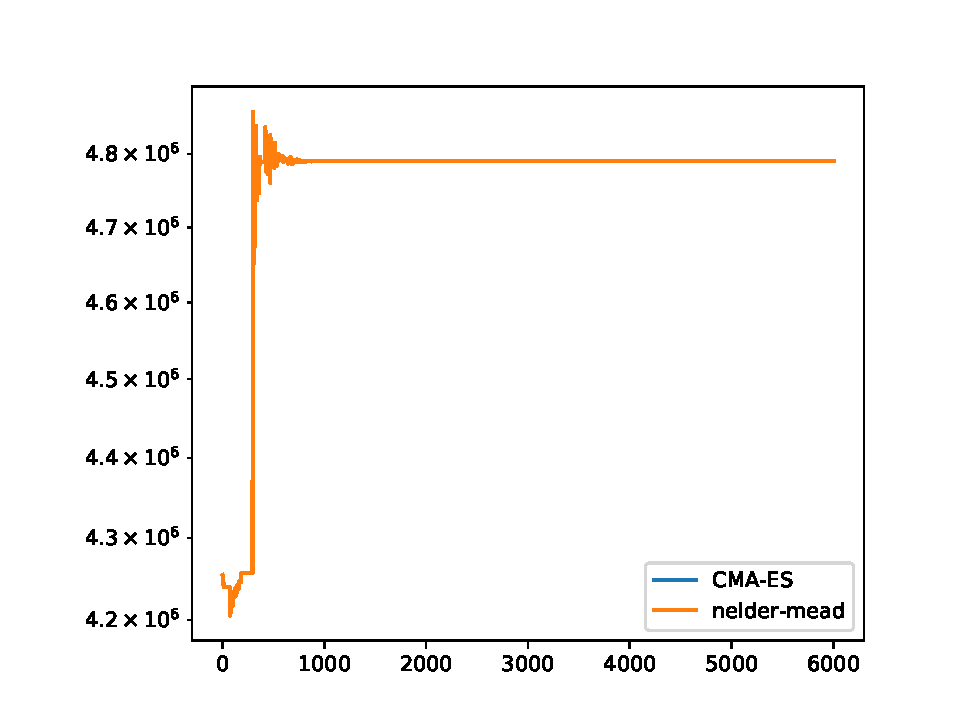
\includegraphics[width=9cm]{cmaes_nelder.pdf}
            \caption{目的関数値の推移}
        \end{figure}
		3005世代からネルダーミード法による最適化がされたが,図3を見る限りCMA-ESとネルダーミード法にはほとんど違いがない.ここで,図4に3005世代以降の目的関数値の推移を示す.縦軸は目的関数値,横軸は世代数または操作回数である.
		\begin{figure}
			\centering
            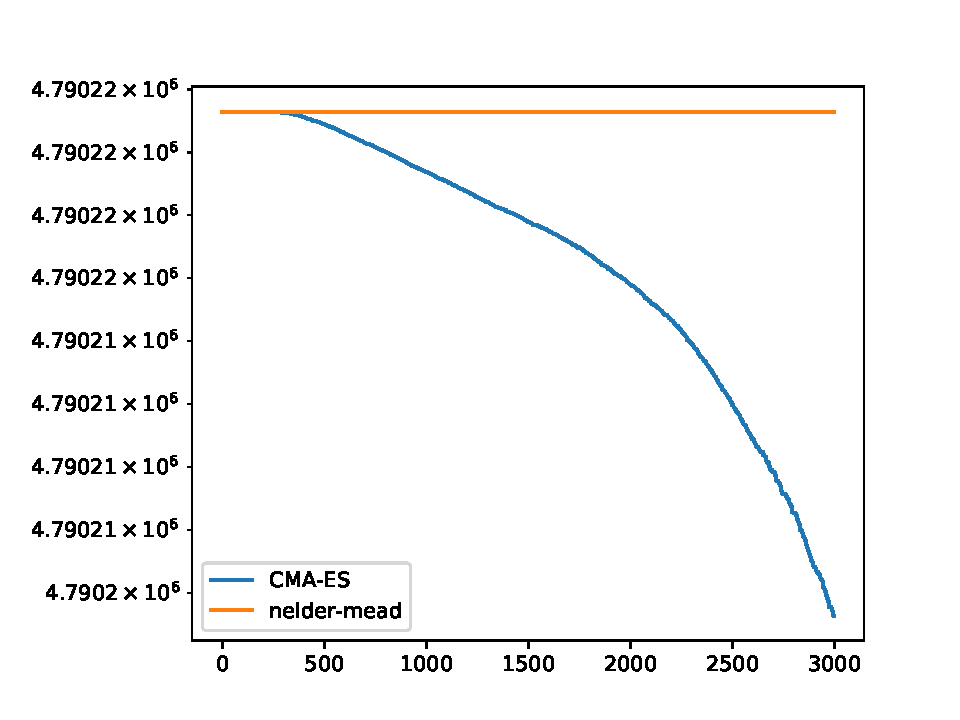
\includegraphics[width=9cm]{cmaes_nelder_v2.pdf}
            \caption{目的関数値の推移}
        \end{figure}
		図4より,CMA-ESの方がネルダーミード法より目的関数を最適化できていることがわかる.
	\subsection{実験2}
		図5に結果として得られた目的関数の推移を示す.縦軸は目的関数値,横軸は世代数と操作回数である.
		\begin{figure}
			\centering
            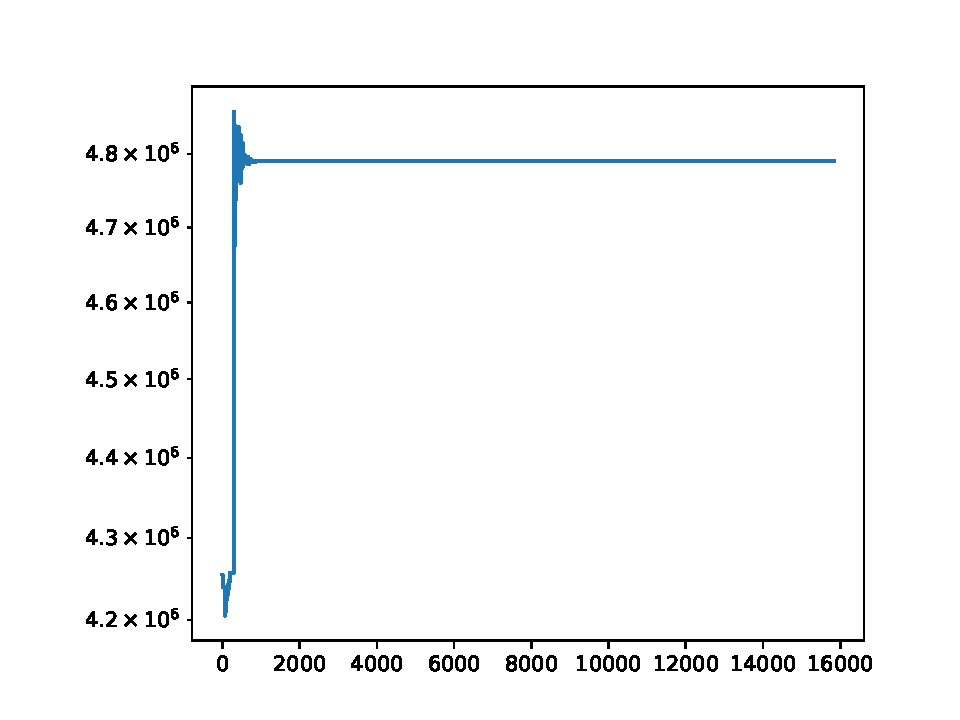
\includegraphics[width=9cm]{cmaes_nelder2.pdf}
            \caption{目的関数値の推移}
        \end{figure}
		図5より,CMA-ESの結果を用いたネルダーミード法は目的関数をほとんど最適化できていないことがわかる.
\section{考察と今後の展望}
	CMA-ESを用いてベンチマーク問題の制約違反を優先して最適化をすると,目的関数値が約480万に落ち着いた.既存の見つかっている解の目的関数値が約400万であることを考えると,一つの局所解にたどり着き抜け出せなくなっている可能性が高い.したがって,ある程度制約違反を許しながら目的関数の最適化をするという方法が考えられる.
	
	また,ネルダーミード法とCMA-ESを組み合わせた最適化として,ネルダーミード法をした後にCMA-ESをするという最適化や,CMA-ESの数世代ごとにネルダーミード法をするという最適化も考えられる.

	さらにCMA-ESのパラメータの調整や,他のバリエーションのCMA-ESも用いてアプローチしたいと考えている.

% 参考文献
\bibliography{hoge}				%hogeはbibファイルのファイル名
\bibliographystyle{junsrt}		%順番に表示

\end{document}